\documentclass{article}
\iffalse
This file is protected by Copyright. Please refer to the COPYRIGHT file
distributed with this source distribution.

This file is part of OpenCPI <http://www.opencpi.org>

OpenCPI is free software: you can redistribute it and/or modify it under the
terms of the GNU Lesser General Public License as published by the Free Software
Foundation, either version 3 of the License, or (at your option) any later
version.

OpenCPI is distributed in the hope that it will be useful, but WITHOUT ANY
WARRANTY; without even the implied warranty of MERCHANTABILITY or FITNESS FOR A
PARTICULAR PURPOSE. See the GNU Lesser General Public License for more details.

You should have received a copy of the GNU Lesser General Public License along
with this program. If not, see <http://www.gnu.org/licenses/>.
\fi

\author{} % Force author to be blank
%----------------------------------------------------------------------------------------
% Paper size, orientation and margins
%----------------------------------------------------------------------------------------
\usepackage{geometry}
\geometry{
	letterpaper,			% paper type
	portrait,				% text direction
	left=.75in,				% left margin
	top=.75in,				% top margin
	right=.75in,			% right margin
	bottom=.75in			% bottom margin
 }
%----------------------------------------------------------------------------------------
% Header/Footer
%----------------------------------------------------------------------------------------
\usepackage{fancyhdr} \pagestyle{fancy} % required for fancy headers
\renewcommand{\headrulewidth}{0.5pt}
\renewcommand{\footrulewidth}{0.5pt}
\newcommand{\terminaloutput}[1]{\texttt{#1}}
\rhead{\small{ANGRYVIPER Team}}
%----------------------------------------------------------------------------------------
% Appendix packages
%----------------------------------------------------------------------------------------
\usepackage[toc,page]{appendix}
%----------------------------------------------------------------------------------------
% Defined Commands & Renamed Commands
%----------------------------------------------------------------------------------------
\renewcommand{\contentsname}{Table of Contents}
\renewcommand{\listfigurename}{List of Figures}
\renewcommand{\listtablename}{List of Tables}
\newcommand{\todo}[1]{\textcolor{red}{TODO: #1}\PackageWarning{TODO:}{#1}} % To do notes
\newcommand{\code}[1]{\texttt{#1}} % For inline code snippet or command line
%----------------------------------------------------------------------------------------
% Various packages
%----------------------------------------------------------------------------------------
\usepackage{hyperref} % for linking urls and lists
\usepackage{graphicx} % for including pictures by file
\usepackage{listings} % for coding language styles
\usepackage{rotating} % for sideways table
\usepackage{pifont}   % for sideways table
\usepackage{pdflscape} % for landscape view
%----------------------------------------------------------------------------------------
% Table packages
%----------------------------------------------------------------------------------------
\usepackage{longtable} % for long possibly multi-page tables
\usepackage{tabularx} % c=center,l=left,r=right,X=fill
\usepackage{float}
\floatstyle{plaintop}
\usepackage[tableposition=top]{caption}
\newcolumntype{P}[1]{>{\centering\arraybackslash}p{#1}}
\newcolumntype{M}[1]{>{\centering\arraybackslash}m{#1}}
%----------------------------------------------------------------------------------------
% Block Diagram / FSM Drawings
%----------------------------------------------------------------------------------------
\usepackage{tikz}
\usetikzlibrary{shapes,arrows,fit,positioning}
\usetikzlibrary{automata} % used for the fsm
%----------------------------------------------------------------------------------------
% Colors Used
%----------------------------------------------------------------------------------------
\usepackage{colortbl}
\definecolor{blue}{rgb}{.7,.8,.9}
\definecolor{ceruleanblue}{rgb}{0.16, 0.32, 0.75}
\definecolor{drkgreen}{rgb}{0,0.6,0}
\definecolor{deepmagenta}{rgb}{0.8, 0.0, 0.8}
\definecolor{cyan}{rgb}{0.0,0.6,0.6}
\definecolor{maroon}{rgb}{0.5,0,0}
%----------------------------------------------------------------------------------------
% Update the docTitle and docVersion per document
%----------------------------------------------------------------------------------------
\def\docTitle{Component Data Sheet}
\def\docVersion{1.5}
%----------------------------------------------------------------------------------------
\date{Version \docVersion} % Force date to be blank and override date with version
\title{\docTitle}
\lhead{\small{\docTitle}}

\def\comp{lime\_adc}
\edef\ecomp{lime_adc}
\def\Comp{Lime ADC}
\graphicspath{ {figures/} }

\begin{document}
\section*{Zipper Deprecation Notice:}
Beginning with OpenCPI Version 1.5, support for Lime Microsystems' Zipper card is now deprecated.
\section*{Summary - \Comp}
\begin{tabular}{|c|M{13.5cm}|}
	\hline
	\rowcolor{blue}
	                  &                  \\
	\hline
	Name              & \comp            \\
	\hline
	Worker Type       & Device           \\
	\hline
	Version           & v\docVersion \\
	\hline
	Release Date      & 4/2019 \\
	\hline
	Component Library & ocpi.assets.devices     \\
	\hline
	Workers           & \comp.hdl        \\
	\hline
	Tested Platforms  &
\begin{itemize}
  \item Epiq Solutions Matchstiq-Z1
  \item Digilent Zedboard/Zipper
  \item x86/Xilinx ML605/Zipper (FMC-LPC/FMC-HPC)
  \item x86/Altera ALST4/Zipper (HSMC A/B)
\end{itemize} \\
	\hline
\end{tabular}

\section*{Functionality}
\begin{flushleft}
	The Lime ADC device worker converts the Lime LMS6002Dr2 Transceiver ADC interface into the OpenCPI WSI interface. The ADC data enters the worker in the sample clock domain (ADC\_CLK) and is registered, de-interleaved, sign-extended, and converted to the control clock domain.
\end{flushleft}

\section*{Worker Implementation Details}
\subsection*{\comp.hdl}
Figure \ref{fig:lime_adc_interface} shows the Lime ADC signal timing interface in the sample clock domain. There are 14 input signals in the interface: ADC\_CLK(1), RX\_IQ\_SEL(1), and RXD(12). The format of the data (RXD) is interleaved complex samples. One data sample (I and Q) is clocked in every two ADC\_CLK cycles with RX\_IQ\_SEL serving as the qualifier for the I sample. The data width for the ADC is 12 bits and the data format is two's complement.\par\bigskip
\begin{figure}[ht]
	\centering
	\includegraphics[scale=.6]{lime_adc_interface}
	\caption{Lime ADC Interface: Sample Clock Domain}
	\label{fig:lime_adc_interface}
\end{figure}
\noindent The clock domain crossing (CDC) from the sample clock to the OpenCPI control clock is performed using a two-clocked synchronizing FIFO with data width of 24 bits and depth of 4096. Data is loaded into the FIFO using RX\_IQ\_SEL and unloaded when the downstream worker is ready. In the event that a sample cannot be loaded into the FIFO, the \verb+overrun+ property is set and remains set until it is cleared. The FIFO output signals are then translated into the WSI interface, which can be seen in Figure \ref{fig:ocpi_adc_interface}. The number of 32 bit complex samples transferred between start-of-message (SOM) and end-of-message (EOM) is set using the worker's \verb+messageSize+ property, where \verb+messageSize+ is in bytes and there are four bytes per complex output sample.\par\bigskip
\begin{figure}[ht]
	\centering
	\includegraphics[scale=.6]{ocpi_adc_interface}
	\caption{WSI Interface: Control Clock Domain}
	\label{fig:ocpi_adc_interface}
\end{figure}
\noindent ADC\_CLK can originate from one of three sources depending on the value of the parameters. The table below describes the valid settings.\par\bigskip
\noindent
\begin{scriptsize}
	\begin{tabular}{|M{4cm}|M{4cm}|M{4cm}|M{4cm}|}
		\hline
		\rowcolor{blue}
		USE\_CLK\_OUT\_p & USE\_CLK\_IN\_p & USE\_CTL\_CLK\_p & ADC\_CLK     \\
		\hline
		True             & X               & X                & RX\_CLK\_OUT \\
		\hline
		False            & True            & X                & RX\_CLK\_IN  \\
		\hline
		False            & False           & True             & ctl\_in.clk  \\
		\hline
	\end{tabular}
\end{scriptsize}\par\bigskip
\noindent RX\_CLK can be driven by this worker by setting the DRIVE\_CLK\_p parameter or it can be driven from another source external to the worker.

\section*{Theory}
The main purpose of this worker is to perform a CDC for a data bus. The decision was made to implement the CDC using a two-clocked FIFO in an effort to target resources native the FPGA.

\section*{Block Diagrams}
\subsection*{Top level}
\begin{center}
	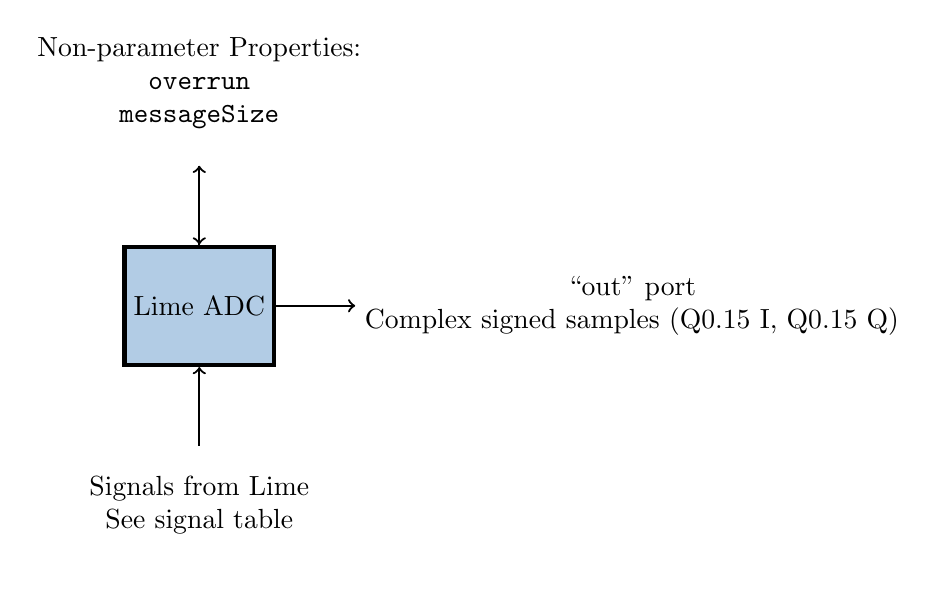
\begin{tikzpicture}[% List of styles applied to all, to override specify on a case-by-case
			every node/.style={
				align=center,  		% use this so that the "\\" for line break works
				minimum size=1.5cm	% creates space above and below text in rectangle
			},
			every edge/.style={draw,thick}
		]
		\node[rectangle,ultra thick,draw=black,fill=blue](R2){\Comp};
		\node[rectangle,draw=white,fill=white](R3)[below= of R2]{Signals from Lime \\ See signal table};
		\node[rectangle,draw=white,fill=white](R4)[right= of R2]{``out'' port \\ Complex signed samples (Q0.15 I, Q0.15 Q)};
		\node[rectangle,draw=white,fill=white](R5)[above= of R2]{Non-parameter Properties:\\\verb+overrun+\\ \verb+messageSize+\\};
		\path[->]
		(R3)edge []	node [] {} (R2)
		(R2)edge []	node [] {} (R4)
		(R2)edge []	node [] {} (R5)
		(R5)edge []	node [] {} (R2)
		;
	\end{tikzpicture}
\end{center}

\section*{Source Dependencies}
\subsection*{\comp.hdl}
\begin{itemize}
	\item assets/hdl/devices/lime\_adc.hdl/lime\_adc.vhd
	\item core/hdl/primitives/util/adc\_fifo.vhd
    \begin{itemize}
    		\item Performs the clock domain crossing from the sample clock to the control clock domain
    \end{itemize}
	\begin{itemize}
		\item core/hdl/primitives/util/sync\_status.vhd
	    \begin{itemize}
    			\item Generates the overrun event when the ADC tries to load a	sample and the ADC FIFO is full
		\end{itemize}
		\item core/hdl/primitives/bsv/imports/SyncFIFO.v
    		\begin{itemize}
		    	\item Two-clocked CDC FIFO
	    \end{itemize}
	\end{itemize}

\end{itemize}
\begin{landscape}

	\section*{Component Spec Properties}
	\begin{scriptsize}
		\begin{tabular}{|p{3.75cm}|p{1.25cm}|p{2cm}|p{2.75cm}|p{1.5cm}|p{1.5cm}|p{1cm}|p{5.25cm}|}
			\hline
			\rowcolor{blue}
			Name               & Type & SequenceLength & ArrayDimensions & Accessibility      & Valid Range & Default & Usage                                                                               \\
			\hline
			\verb+messageSize+ & Long & -              & -               & Initial, Readable  & Standard    & -       & Number of bytes in output message                                                   \\
			\hline
			\verb+overrun+     & Bool & -              & -               & Writable, Volatile & Standard    & -       & Flag set when ADC tries to load a sample and the ADC FIFO is full. Once high, this flag is not cleared (i.e. set low) until the property is written to again (the flag clears regardless of write value, i.e. writing true or false both result in a value of false, also note that a property write happens on reset).\\
			\hline
		\end{tabular}
	\end{scriptsize}

	\section*{Worker Properties}
	\subsection*{\comp.hdl}
	\begin{scriptsize}
		\begin{tabular}{|p{2cm}|p{2cm}|p{1cm}|c|c|c|c|c|p{6.5cm}|}
			\hline
			\rowcolor{blue}
			Type         & Name                 & Type & SequenceLength & ArrayDimensions & Accessibility & Valid Range        & Default & Usage                                                                                                                  \\
			\hline
			Property     & \verb+other_present+ & Bool & -              & -               & Readable      & -                  & -       & Not implemented. Flag to indicated presence of DAC worker                                                              \\
			\hline
			Property     & \verb+DRIVE_CLK_p+   & Bool & -              & -               & Parameter     & Standard           & 1       & Drive the clock sent to Lime (RX\_CLK). Some platforms do not connect RX\_CLK to the FPGA, making this parameter false \\
			\hline
			Property     & \verb+USE_CLK_IN_p+  & Bool & -              & -               & Parameter     & Standard           & 0       & Use copy of clock sent to Lime (RX\_CLK) as ADC\_CLK. Not guaranteed to be aligned with RX data                        \\
			\hline
			Property     & \verb+USE_CTL_CLK_p+ & Bool & -              & -               & Parameter     & Standard           & 1       & Use control clock as ADC\_CLK. This is primarily for testing the component.                                            \\
			\hline
			Property     & \verb+divisor+       & -    & -              & -               & Writable      & -                  & -       & Not implemented. Divider for ADC clock. This is primarily for testing the component.                                   \\
			\hline
			Property     & \verb+USE_CLK_OUT_p+ & Bool & -              & -               & Parameter     & Standard           & 1       & Use clock output from Lime (RX\_CLK\_OUT) as ADC\_CLK. RX\_CLK\_OUT is aligned with RX data                            \\
			\hline
			Property     & \verb+source+        & Enum & -              & -               & Initial       & adc,count,loopback & adc     & Not implemented. Runtime property to indicate worker parameter configuration                                           \\
			\hline
			SpecProperty & \verb+messageSize+   & -    & -              & -               & -             & -                  & 8192    & Number of bytes in output message                                                                                      \\
			\hline
			SpecProperty & \verb+overrun+       & -    & -              & -               & -             & -                  & 0       & Flag set when ADC tries to load a sample and the ADC FIFO is full. Once high, this flag is not cleared (i.e. set low) until the property is written to again (the flag clears regardless of write value, i.e. writing true or false both result in a value of false, also note that a property write happens on reset).                                   \\
			\hline
		\end{tabular}
	\end{scriptsize}

	\section*{Component Ports}
	\begin{scriptsize}
		\begin{tabular}{|p{2cm}|p{1.5cm}|p{4cm}|p{1.5cm}|p{1.5cm}|p{9.38cm}|}
			\hline
			\rowcolor{blue}
			Name & Producer & Protocol           & Optional & Advanced & Usage                  \\
			\hline
			out  & true     & iqstream\_protocol & true     & -        & Complex signed samples (Q0.15 I, Q0.15 Q). \\
			\hline
		\end{tabular}
	\end{scriptsize}
\pagebreak
	\section*{Worker Interfaces}
	\subsection*{\comp.hdl}
	\begin{scriptsize}
		\begin{tabular}{|p{2cm}|p{1.5cm}|p{1.5cm}|p{1.5cm}|p{13.8cm}|}
			\hline
			\rowcolor{blue}
			Type            & Name & DataWidth & Advanced & Usage                  \\
			\hline
			StreamInterface & out  & 32        & -        & Complex signed samples (Q0.15 I, Q0.15 Q). This port generates data and obeys backpressure. Because both backpressure from the \verb+out+ port and forward pressure from the \verb+dev_adc+ data bus exists, it is possible for samples to be dropped in the clock domain-crossing FIFO, i.e. seen on the \verb+dev_adc+ data bus but never make it to the output port. This event is monitored via the \verb+overrun+ property.  \\
			\hline
		\end{tabular}
	\end{scriptsize}

	\section*{Signals}
	\begin{scriptsize}
		\begin{tabular}{|M{2.5cm}|M{1.5cm}|M{1.5cm}|M{14.5cm}|}
			\hline
			\rowcolor{blue}
			Name         & Type   & Width & Description                       \\
			\hline
			RX\_CLK      & Output & 1     & Clock input to Lime               \\
			\hline
			RX\_CLK\_OUT & Input  & 1     & Clock output from Lime            \\
			\hline
			RX\_IQ\_SEL  & Input  & 1     & IQ Select from Lime               \\
			\hline
			RXD          & Input  & 12    & Lime ADC data bus. IQ interleaved \\
			\hline
			RX\_CLK\_IN  & Input  & 1     & Copy of RX\_CLK sent to FPGA      \\
			\hline
		\end{tabular}
	\end{scriptsize}
\end{landscape}

\section*{Control Timing and Signals}
The Lime ADC device worker uses the clock from the Control Plane and Control Plane signals.\par\bigskip
\noindent The latency through the worker from the ADC pins to the output port is 2 sample clock cycles and 1 control clock cycle. The data is registered twice in the sample clock domain (once to capture the ADC pins, and once to capture I and Q) before it is loaded into the CDC FIFO.

\begin{landscape}
\section*{Worker Configuration Parameters}
\subsubsection*{\comp.hdl}
%\input{../../\ecomp.hdl/configurations.inc}
\section*{Performance and Resource Utilization}
\subsubsection*{\comp.hdl}
The table entries for configuration ``0'' are a result of building the worker for the following (Matchstiq-Z1-related) parameter set. Note that that are two global clocks (GCLKs), one for the control plane clock, and one for the Lime ADC-sourced clock (Fmax is assumed to be worst case for all available clocks).\\

The Virtex-6 implementation is specific to the Zipper card's pin locations, which exhibit suboptimal timing due to the Lime ADC's clock pin location on the FPGA. Table entries for configuration1 ``1'' are a result of building the worker for the (Zipper-related) parameter set.\\

%\input{../../\ecomp.hdl/utilization.inc}
\end{landscape}
\section*{Test and Verification}
\begin{flushleft}
 To be detailed in a future release.
\end{flushleft}
\section*{References}
\begin{flushleft}
	\begin{itemize}
		\item[1)] LMS6002D Datasheet, www.limemicro.com
	\end{itemize}
\end{flushleft}
\end{document}
